\documentclass[border=2mm]{standalone}
\usepackage{csquotes}
\usepackage[backend=biber,style=numeric,sorting=none]{biblatex}
 
\usepackage{siunitx}
\usepackage{tikz}
\usetikzlibrary{decorations.pathmorphing,patterns}
\usetikzlibrary{shapes.geometric, arrows}
\usetikzlibrary{positioning}
 
\usepackage{amsmath}
 
\usepackage{tikz-3dplot}
\usetikzlibrary{3d}
 
\usepackage[siunitx,american]{circuitikz}
 
\usepackage{pgfplots}
\usepgfplotslibrary{units}
\usepgfplotslibrary{groupplots}
\pgfplotsset{compat=1.14}
 
\ctikzset{tripoles/mos style/arrows}

\definecolor{IBM1}{HTML}{648fff}
\definecolor{IBM2}{HTML}{785ef0}
\definecolor{IBM3}{HTML}{dc267f}
\definecolor{IBM4}{HTML}{fe6100}
\definecolor{IBM5}{HTML}{ffb000}
\definecolor{IBM6}{HTML}{d55e00}
\definecolor{IBM7}{HTML}{cc79a7}
\definecolor{IBM8}{HTML}{0072b2}
\definecolor{IBM9}{HTML}{f0e442}
\definecolor{IBM10}{HTML}{009e73}

\begin{document}

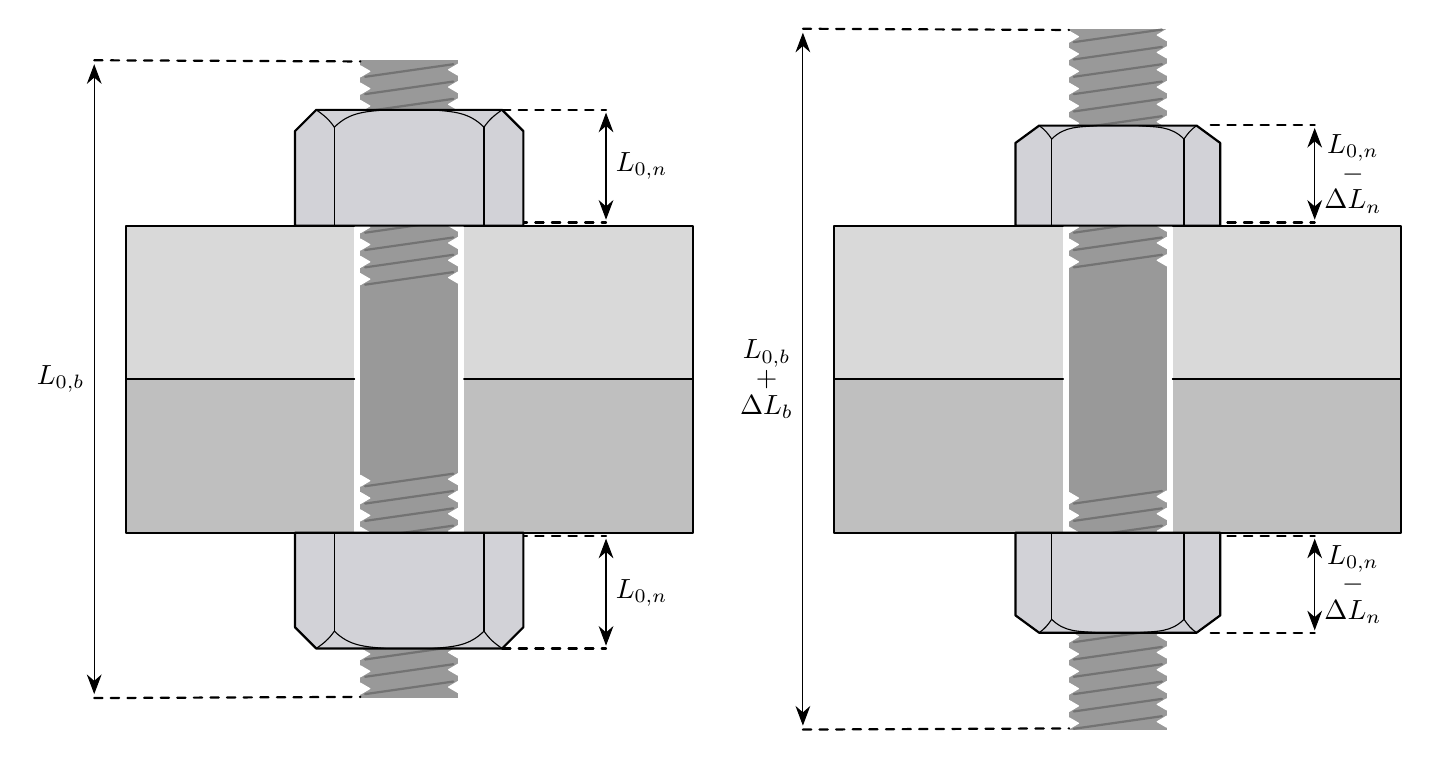
\begin{tikzpicture}[line join=round, line cap=round]

\definecolor{metalLight}{RGB}{230,230,235}
\definecolor{metalDark}{RGB}{120,120,130}
\definecolor{nutFill}{RGB}{210,210,215}
\definecolor{nutEdge}{RGB}{165,165,172}
\definecolor{nutSide}{RGB}{178,178,185}
\definecolor{nutCenter}{RGB}{222,222,228}
\definecolor{nutTopFace}{RGB}{202,202,208}

\def\threadHeight{3.5}
\def\threadIntoPlate{0.75}
\pgfmathtruncatemacro{\threadSteps}{\threadHeight/0.22}

%flanke
\fill[gray!30] (-3.6,0) rectangle (-0.70,1.95);
\fill[gray!30] (0.70,0) rectangle (3.6,1.95);
\fill[gray!50] (-3.6,-1.95) rectangle (-0.70,0);
\fill[gray!50] (0.70,-1.95) rectangle (3.6,0);
\draw[thick] (-0.70,0)--(-3.6,0)--(-3.6,1.95)--(-0.70,1.95);
\draw[thick] (-0.70,0)--(-3.6,0)--(-3.6,-1.95)--(-0.70,-1.95);
\draw[thick] (0.70,0)--(3.6,0)--(3.6,1.95)--(0.70,1.95);
\draw[thick] (0.70,0)--(3.6,0)--(3.6,-1.95)--(0.70,-1.95);

%bolt
\fill[gray!80] (-0.62,-4.05) rectangle (0.62,4.05);

%thread
\foreach \k [evaluate=\k as \y using {1.95-\threadIntoPlate + \k*0.22}] in {0,...,12} {
	\draw[line width=0.8pt, black!55] (-0.56,\y) -- (0.56,\y+0.16);
	\filldraw[fill=white, draw=white] (-0.62,\y) -- (-0.62,\y+0.14) -- (-0.50,\y+0.07) -- cycle;
	\filldraw[fill=white, draw=white] (0.62,\y+0.02) -- (0.62,\y+0.16) -- (0.50,\y+0.09) -- cycle;
}
\foreach \k [evaluate=\k as \y using {-(1.95-\threadIntoPlate + 0.16 + \k*0.22)}] in {0,...,12} {
	\draw[line width=0.8pt, black!55] (-0.56,\y) -- (0.56,\y+0.16);
	\filldraw[fill=white, draw=white] (-0.62,\y) -- (-0.62,\y+0.14) -- (-0.50,\y+0.07) -- cycle;
	\filldraw[fill=white, draw=white] (0.62,\y+0.02) -- (0.62,\y+0.16) -- (0.50,\y+0.09) -- cycle;
}

% tegninger
\draw[dashed, thick] (-4,4.05) -- (-0.62,4.035);
\draw[dashed, thick] (-4,-4.05) -- (-0.62,-4.035);
\draw[-{Stealth[length=2.5mm]}] (-4,0) -- (-4,-4);
\draw[-{Stealth[length=2.5mm]}] (-4,0) -- (-4,4);
\node[anchor=east] at (-4,0) {$L_{0,b}$};

\draw[dashed, thick] (1.18,3.42) -- (2.5,3.42);
\draw[dashed, thick] (1.18,1.99) -- (2.5,1.99);
\draw[dashed, thick] (1.18,-3.42) -- (2.5,-3.42);
\draw[dashed, thick] (1.18,-1.99) -- (2.5,-1.99);
\draw[-{Stealth[length=2.5mm]}] (2.5,2.71) -- (2.5,3.42-0.035);
\draw[-{Stealth[length=2.5mm]}] (2.5,2.71) -- (2.5,1.99+0.035);
\draw[-{Stealth[length=2.5mm]}] (2.5,-2.71) -- (2.5,-3.42+0.035);
\draw[-{Stealth[length=2.5mm]}] (2.5,-2.71) -- (2.5,-1.99-0.035);
\node[anchor=west] at (2.5,2.71) {$L_{0,n}$};
\node[anchor=west] at (2.5,-2.71) {$L_{0,n}$};

%top nut
\fill[nutFill] (-1.45,1.95) -- (1.45,1.95) --
(1.45,3.15) -- (1.18,3.42) -- (-1.18,3.42) -- (-1.45,3.15) -- cycle;
\draw[thick] (-1.45,1.95) -- (1.45,1.95) --
(1.45,3.15) -- (1.18,3.42) -- (-1.18,3.42) -- (-1.45,3.15) -- cycle;
\draw[black] (-0.95,3.2) -- (-0.95,1.95);
\draw[black] (0.95,3.2) -- (0.95,1.95);
\draw[black] (-1.18,3.42) to[out=-35,in=125] (-0.95,3.2);
\draw[black] (1.18,3.42) to[out=-145,in=55] (0.95,3.2);
\draw[black] (-0.95,3.2) to[out=45,in=-175] (-0.3,3.42);
\draw[black] (0.3,3.42) to[out=-5,in=-225] (0.95,3.2);

%bot nut
\fill[nutFill] (-1.45,-1.95) -- (1.45,-1.95) --
(1.45,-3.15) -- (1.18,-3.42) -- (-1.18,-3.42) -- (-1.45,-3.15) -- cycle;
\draw[thick] (-1.45,-1.95) -- (1.45,-1.95) --
(1.45,-3.15) -- (1.18,-3.42) -- (-1.18,-3.42) -- (-1.45,-3.15) -- cycle;
\draw[black] (-0.95,-3.2) -- (-0.95,-1.95);
\draw[black] (0.95,-3.2) -- (0.95,-1.95);
\draw[black] (-1.18,-3.42) to[out=35,in=-125] (-0.95,-3.2);
\draw[black] (1.18,-3.42) to[out=145,in=-55] (0.95,-3.2);
\draw[black] (-0.95,-3.2) to[out=-45,in=175] (-0.3,-3.42);
\draw[black] (0.3,-3.42) to[out=5,in=225] (0.95,-3.2);

\begin{scope}[xshift=9cm]
%flanke
\fill[gray!30] (-3.6,0) rectangle (-0.70,1.95);
\fill[gray!30] (0.70,0) rectangle (3.6,1.95);
\fill[gray!50] (-3.6,-1.95) rectangle (-0.70,0);
\fill[gray!50] (0.70,-1.95) rectangle (3.6,0);
\draw[thick] (-0.70,0)--(-3.6,0)--(-3.6,1.95)--(-0.70,1.95);
\draw[thick] (-0.70,0)--(-3.6,0)--(-3.6,-1.95)--(-0.70,-1.95);
\draw[thick] (0.70,0)--(3.6,0)--(3.6,1.95)--(0.70,1.95);
\draw[thick] (0.70,0)--(3.6,0)--(3.6,-1.95)--(0.70,-1.95);

%bolt
\fill[gray!80] (-0.62,-4.45) rectangle (0.62,4.45);

%thread
\foreach \k [evaluate=\k as \y using {1.95-\threadIntoPlate + 0.22 + \k*0.22}] in {0,...,13} {
	\draw[line width=0.8pt, black!55] (-0.56,\y) -- (0.56,\y+0.16);
	\filldraw[fill=white, draw=white] (-0.62,\y) -- (-0.62,\y+0.14) -- (-0.50,\y+0.07) -- cycle;
	\filldraw[fill=white, draw=white] (0.62,\y+0.02) -- (0.62,\y+0.16) -- (0.50,\y+0.09) -- cycle;
}
\foreach \k [evaluate=\k as \y using {-(1.95-\threadIntoPlate + 0.16 + 0.22 + \k*0.22)}] in {0,...,13} {
	\draw[line width=0.8pt, black!55] (-0.56,\y) -- (0.56,\y+0.16);
	\filldraw[fill=white, draw=white] (-0.62,\y) -- (-0.62,\y+0.14) -- (-0.50,\y+0.07) -- cycle;
	\filldraw[fill=white, draw=white] (0.62,\y+0.02) -- (0.62,\y+0.16) -- (0.50,\y+0.09) -- cycle;
}

% tegninger
\draw[dashed, thick] (-4,4.45) -- (-0.62,4.435);
\draw[dashed, thick] (-4,-4.45) -- (-0.62,-4.435);
\draw[-{Stealth[length=2.5mm]}] (-4,0) -- (-4,-4.4);
\draw[-{Stealth[length=2.5mm]}] (-4,0) -- (-4,4.4);
\node[anchor=east,align=center] at (-4,0) {$L_{0,b}$\\[-2pt]$+$\\[-2pt]$\Delta L_b$};

\draw[dashed, thick] (1.18,3.225) -- (2.5,3.225);
\draw[dashed, thick] (1.18,1.99) -- (2.5,1.99);
\draw[dashed, thick] (1.18,-3.225) -- (2.5,-3.225);
\draw[dashed, thick] (1.18,-1.99) -- (2.5,-1.99);
\draw[-{Stealth[length=2.5mm]}] (2.5,2.6075) -- (2.5,3.225-0.035);
\draw[-{Stealth[length=2.5mm]}] (2.5,2.6075) -- (2.5,1.99+0.035);
\draw[-{Stealth[length=2.5mm]}] (2.5,-2.6075) -- (2.5,-3.225+0.035);
\draw[-{Stealth[length=2.5mm]}] (2.5,-2.6075) -- (2.5,-1.99-0.035);
\node[anchor=west,align=center] at (2.5,2.6075) {$L_{0,n}$\\[-2pt]$-$\\[-2pt]$\Delta L_n$};
\node[anchor=west,align=center] at (2.5,-2.6075) {$L_{0,n}$\\[-2pt]$-$\\[-2pt]$\Delta L_n$};

%top nut
\fill[nutFill] (-1.30,1.95) -- (1.30,1.95) --
(1.30,3.00) -- (1.00,3.22) -- (-1.00,3.22) -- (-1.30,3.00) -- cycle;
\draw[thick] (-1.30,1.95) -- (1.30,1.95) --
(1.30,3.00) -- (1.00,3.22) -- (-1.00,3.22) -- (-1.30,3.00) -- cycle;
\draw[black] (-0.84,3.05) -- (-0.84,1.95);
\draw[black] (0.84,3.05) -- (0.84,1.95);
\draw[black] (-1.00,3.22) to[out=-35,in=125] (-0.84,3.05);
\draw[black] (1.00,3.22) to[out=-145,in=55] (0.84,3.05);
\draw[black] (-0.84,3.05) to[out=45,in=-175] (-0.26,3.22);
\draw[black] (0.26,3.22) to[out=-5,in=-225] (0.84,3.05);

%bot nut
\fill[nutFill] (-1.30,-1.95) -- (1.30,-1.95) --
(1.30,-3.00) -- (1.00,-3.22) -- (-1.00,-3.22) -- (-1.30,-3.00) -- cycle;
\draw[thick] (-1.30,-1.95) -- (1.30,-1.95) --
(1.30,-3.00) -- (1.00,-3.22) -- (-1.00,-3.22) -- (-1.30,-3.00) -- cycle;
\draw[black] (-0.84,-3.05) -- (-0.84,-1.95);
\draw[black] (0.84,-3.05) -- (0.84,-1.95);
\draw[black] (-1.00,-3.22) to[out=35,in=-125] (-0.84,-3.05);
\draw[black] (1.00,-3.22) to[out=145,in=-55] (0.84,-3.05);
\draw[black] (-0.84,-3.05) to[out=-45,in=175] (-0.26,-3.22);
\draw[black] (0.26,-3.22) to[out=5,in=225] (0.84,-3.05);

\end{scope}

\end{tikzpicture}

\end{document}